\documentclass{article}
\usepackage{graphicx} % Required for inserting images
\usepackage{enumitem} % for customisible enumerators
\usepackage{float} % for text under pictures
\usepackage[colorlinks=true, linkcolor=black]{hyperref} % for links in refs
\usepackage{cleveref} % for easier referencing
\usepackage{caption} % easier captioning for tables
\captionsetup[table]{position=above}

\title{Vilnius University\\Faculty of Mathematics and Informatics\\Software Engineering\\3rd course\\[1cm] \Huge Universal PoS application for small to medium-sized businesses\\[1cm]}
\author{\textbf{PoS application [Tuesday 12 pm]}\\[0.25cm]Rytis Tauras\\Matas Čeplinkas\\Emil Duko\\Žygimantas Vidmantas\\Rytis Jonika\\[4cm]}
\date{September 2025}

\usepackage{titlesec}
\newcounter{subsubsubsection}[subsubsection]
\renewcommand\thesubsubsubsection{\thesubsubsection.\arabic{subsubsubsection}}

\newcommand\subsubsubsection[1]{
  \refstepcounter{subsubsubsection}
  \paragraph{\thesubsubsubsection\quad #1}
}

\begin{document}

\maketitle

\newpage
\setcounter{tocdepth}{3}
\tableofcontents
\newpage

\section{Introduction}
\subsection{Software title}
\subsubsection{Full title} Universal POS application for small to medium-sized businesses
\subsubsection{Short title} POS application
\subsection{Problem statement}  Today, the need for a reliable point-of-sale (PoS) system is greater than ever before. Due to fast pace and increasing client traffic, companies and their employees that use PoS systems face the challenge of unreliable and inefficient systems.
\par To be more precise, PoS operators that work hand in hand with the system often struggle with unexpected errors, lack of functionality, difficult to navigate user interfaces, slow processing, and inefficient workflow, all of which cause unwanted stress on a daily basis. Furthermore, it also has a negative effect on new business owners because starting a business takes more time, and usually they have to sort through different systems to find the best fit, which results in consumption of significant part of funding for installation and employee training. The clients of these companies are highly dependent on the quality of service, and these faulty systems directly contribute to longer wait times and a general decrease in the quality of the provided service.
\par These challenges mostly arise in cafes, bars, restaurants, spas, and other settings where smooth workflow between sales, reservations, and management is crucial - the hospitality sector. Firstly, the root of the problem usually lies in poor synchronization between different departments, for example, warehouse and sales, when customer tries ordering a product but the system fails to notify that it is out of stock. Secondly, another hindering factor is that most PoS systems support only a single language menu or user interface, which causes problems for international workers. Another problem is confusing or unintuitive user interfaces.
\par All of these problems occur during work hours and preparations, causing delays and mistakes. It is important to address this problem because faulty PoS systems hinder business processes by decreasing profit, resulting in financial losses. It also reduces customer satisfaction, causing customers to have mistrust, which builds barriers for new businesses or enhances frustration for more established business owners and their employees.
\newpage

\section{User needs analysis}
\subsection{Expectations of the stakeholders}
\subsubsection{Primary stakeholders}
\textbf{POS operators} expect to have a system for fulfilling orders and making appointments that:
\begin{itemize}
    \item Has high transaction efficiency
    \item Reduces errors
    \item Helps provide quick assistance to customers
    \item Has minimal training and is easy to remember
    \item Has smooth integration of appointment system
    \item Allows resource monitoring
    \item Supports card, cash and gift-card payments
    \item Supports multiple languages.
\end{itemize}


\subsubsection{Secondary stakeholders}

\textbf{Clients} expect the order/appointments to be accurately delivered and without delays, as well as to have the option of splitting the bill, receive an invoice and refund an order or service.
\textbf{\\ Other employees} expect the system to be reliable, so as not to interrupt their own work. A solution is needed which allows other employees to view appointments assigned to them in their own devices.
\textbf{\\ Business managers} require an intuitive system for managing products, pricing, discounts, and employees within the system.

\subsubsection{Tertiary stakeholders}

\textbf{Business owners} expect a system that serves customers faster, is error-free, is adaptable to their business model, can be integrated onto current systems and into current workflows seamlessly, and does not require lengthy training sessions for PoS operators.
\newpage

\subsubsection{Competitors}The closest competitors available to PoS application are:
\begin{itemize}
    \item \textbf{Paysera POS}
    \\Paysera POS is a widely applicable, feature-rich system with an intuitive and modern user interface.
    \item \textbf{WinPOS}
    \\WinPOS offers installation with Windows Embedded POSready system, and offers multi-language support.
    \item \textbf{iiko}
    \\iiko offers multiple restaurant-oriented POS systems according to the specific process, and offers comprehensive operation statistics to customer.
    \item \textbf{r\_keeper}
    \\r\_keeper offers a simplistic POS system for restaurants with an updated user interface.
    \item \textbf{nSoft nPoint}
    \\n\_soft provides a comprehensive POS system for many organization types, with support for third-party programs.
\end{itemize}
The main advantages of our PoS application are multi-language UI (beyond Lithuanian and English) support, ability to translate menus, and easier to learn and use user interface and more affordable service.
\subsubsection{Developers \& maintenance team}
Team responsible for maintenance and development expects a system that can be scaled or adjusted if business model of PoS system's customer changes. Additionally, it should be maintainable without dedicating more than one person to keep things running.  
\newpage
\subsection{POS operators research}
\subsubsection{Current users' activities}

\subsubsubsection{Unknown language borders}
\label{Unknow language borders}
\paragraph{\small Story:} Carlos and Juan, two older gentleman from Spain, have joined a popular Lithuanian specialty coffee place. Both of them speak Spanish, Carlos knows English. They have extensive knowledge about coffees and more than 30 years of experience in the field. This experience does not translate well to their order taking speed, as the system has English and Lithuanian user-interface options, and the menu of beverages and food items is available only in Lithuanian language. Carlos has set the user interface to English, so he has no problem understanding the systems order flow, but both Carlos and Juan struggle with selecting items from Lithuanian menu in the system. Despite their experience, this has significantly impacted their work efficiency. Instead of a few seconds to add an item to an order on the touch screen PoS system, while they learn the menu, it takes more than 20 seconds to remember the item's name in Lithuanian language. Juan struggles with remembering different terms in the check out menu. He has learned basic order flow (creating a new order, selecting payment, etc), but when he needs to perform a rare action (such as refunding or splitting the order), he gets stuck and needs to get help from other employees. The average total order taking time increases from less than a minute to over 2 minutes (Not counting time to make and serve the order). The coffee place sells hundreds of beverages and other items per day, and this delay adds up to a significant amount causing slower service and dissatisfied customers.

\paragraph{\small Problems and Opportunities:} The problem is caused by the fact that the current PoS system only supports a single language item menu and two language user-interface.\\ An opportunity would be to develop a system with a broad selection of languages for the user interface and an option to add translation to the menu items in needed language.

\subsubsubsection{Stock management failure}
\label{Stock management failure}
\paragraph{\small Story:} Twenty-year-old student Laura is a new hire in a take-away burger joint. After a short introduction to the PoS system, she starts taking customer orders. It is a busy Friday night. She listens to an order from a customer and enters it into the system, a burger with cheese and bacon. The customer leaves and waits for the order outside of the place. Laura starts taking another customers' orders when 10 minutes later an angry chef comes out to the front and shouts at Laura that they are out of bacon and that she should have asked them before confirming the order. Now Laura needs to run outside, find the customer and offer to order again while the previous order is refunded or to get a partial discount and get the burger without bacon. The customer is angry since they have already waited a total of 15 minutes and now the order will take even longer. While Laura tries to de-escalate the situation a long, noisy queue forms.
\paragraph{\small Problems and Opportunities:} The problem was caused by the fact that the current PoS system does not have an integrated stock management system.\\ An opportunity would be to design the system that would track the inventory.

\subsubsubsection{Failed customer assistance}
\label{Failed customer assistance}
\paragraph{\small Story:} Trevor is a fifty year old who works at a restaurant part time. While getting an order he gets asked about the list of ingredients used in the cake that the customer wants to order, specifically whether it contains any traces of nuts because the customer is severely allergic to them. Trevor is not sure about the answer, so he tries looking for that information in his ordering system, but he is not able to find any. He struggles with handling the system, because he did not grow up with this kind technology at hand. Then he decides to go to the product manager for more information, however his office is in the back corner of the restaurant so Trevor has to go through the kitchen to reach it. This action results in Trevor having to drop his work and taking up 5 minutes of his and the customers' time while also hindering the build of trust between restaurants' customers.
\paragraph{\small Problems and Opportunities:} The problem was caused by not having means to get additional information (ingredients and descriptions) in the PoS system or having it implemented in a way that inexperienced PoS operators could not find it.\\ An opportunity would be to design the PoS system that has easy to find information to any anticipated questions that the customer might come up with without having to involve any other employees.

\subsubsubsection{Receipt management}
\label{Receipt management}
\paragraph{\small Story:} Renata is a 32-year-old waiter working in a high-end restaurant. During a business dinner, one of the two attending parties, in a hurry, request to pay and have the bill split according to the ordered food, and have an invoice sent to their e-mail. The in-use PoS system, "nPoint", supports only receipt splitting, but not forwarding invoices through e-mail. Because of this, Renata has to inform the customers that the invoice can only be printed out, or that the manually send an e-mail in one to two business days. The customer has to choose the inconvenience of waiting for the invoice to arrive, or take the printed invoice, and risk damaging or losing it. The customer chooses to take the physical invoices, and is dissatisfied with the restaurant.

\paragraph{Problems and Opportunities:} The problem arises when clients requests an invoice for their order in a non-physical format, which is only supported by one other provider, which does not fit the needs of the high-end restaurant.\\The ability to send invoices through e-mail in the PoS application is a great option when the customer is short on time, and generally is more convenient than a printed invoice. An additional opportunity is to have support for order-splitting at any given time during the orders lifespan, as customers may request to pay and leave separately.

\subsubsection{Characteristics of people, activities, context, and technologies}
\paragraph{\small People:} Mostly young hospitality workers varied in ethnic backgrounds who have high motivation to succeed, with the exception of some elderly ones not so handy with technology, some of whom lack sufficient training or struggle with the language barrier of the system.
\paragraph{\small Activities:} Daily high pressure and quick response time work consisting of handling order input and searching for important information - sometimes stressful safety critical situations where customers health could be at risk. The main goal is to do your job as quickly and as correctly as possible.
\paragraph{\small Context:} Physical environment is loud, quite warm or even hot near the kitchen area, filled with a variety of chatter and smells. The space where the workers manage the orders system is well lit, but the main dining area is lit quite dimly. Social environment consists of constant interactions with customers and work colleagues as well as individual concern of getting orders correctly.
\paragraph{\small Technologies:} A touch screen interface facing the worker to input orders, edit them or close tabs. Printer for checks and hand card terminal for cashless transactions.

% add main functions like login and cancel, refund etc (function list)
\subsubsection{Needs}
\begin{enumerate}[label=N\arabic*.]
    \item Carlos and Juan need a system that supports item menu translation in the PoS system, so they would not need to learning and remember foreign language names during the working-hours in the coffee shop. This would significantly reduce their learning efficiency.
    \item Juan needs a system that supports a wider user-interface language selection, to ensure he does not get stuck not knowing how to navigate the system during order taking, especially with unusual requests.
    \item Carlos and Juan need to be able to use the search to find items in their native language, so they can find items quickly and without need to memorize foreign item names.
    \item Laura needs a system that shows the remaining product stock during order entry into the system. She would not need to confirm with chefs that there are enough products for the order, therefore saving customers and hers time.
    \item Laura needs a system in which it is possible to enter the remaining product stock during stock-taking or when needed so that an accurate inventory situation is portrayed during service hours, in order to know which items are still available for sale.
    \item Laura needs a system that decrements the remaining product stock after each sale during service and gives a warning when certain item reaches a set (adjustable) near out-of-stock amount. This would prevent selling an item that is out of stock or near it without noticing.
    \item Trevor needs the system to provide needed information about menu items, such as their ingredients and descriptions, so he could provide feedback to customers' questions without having to ask the manager.
    \item Trevor needs an understandable interface to retrieve information about menu items, so he can quickly find and provide needed information to the inquiring customer. 
    \item Renata needs a PoS system that can quickly produce an invoice for a specific order and have options to print out or send the receipt according to customer request.
    \item Renata needs a capability to swiftly split up a specific order into multiple orders at any given time in an order's lifetime.
\end{enumerate}

\begin{table}[h]
\centering
\caption{Traceability matrix for PoS operators needs and stories they stem from}
\begin{tabular}{|c|c|}
\hline
\textbf{Need ID} & \textbf{Story number} \\ \hline
N1  & \ref{Unknow language borders} \\ \hline
N2  & \ref{Unknow language borders} \\ \hline
N3  & \ref{Unknow language borders} \\ \hline
N4  & \ref{Stock management failure} \\ \hline
N5  & \ref{Stock management failure} \\ \hline
N6  & \ref{Stock management failure} \\ \hline
N7  & \ref{Failed customer assistance} \\ \hline
N8  & \ref{Failed customer assistance} \\ \hline
N9  & \ref{Receipt management} \\ \hline
N10 & \ref{Receipt management} \\ \hline
\end{tabular}
\end{table}

\subsubsection{Usability objectives}
\begin{enumerate}[label=S\arabic*.]
    \item Learnability: 95\% of foreign workers will be able to perform the basic and unusual PoS flows (order taking, different payment methods, refunds, check splitting, etc.) in less than 1 hour of training, if the user interface and item menu supports their native language.
    \item Satisfaction: At least 80\% of foreign PoS system operators will rate the system as 'satisfactory' or better (more than 4 on a 5-point scale) after a week of work with the system, if it is available in their language.
    \item Memorability: At least 95\% of foreign workers will be able to complete unusual tasks during service (refunds, check splitting, providing information) after not using the PoS system for more than a week.
    \item Errors: If the inventory amounts are entered correctly, 100\% of the orders taken by the PoS operator will reach the buyer (having enough stock).
    \item Efficiency: PoS system operating employee should be able to find an answer to a question in 30 seconds or less, if the information is disclosed in the system.
    \item Learnability: 90\% of Employees should be able to learn the use of system in 30 minutes or less.
    \item Learnability: At least  90\% of PoS operators that have received 30 minutes of training on the system will be able to split an order by customers request and send an invoice to their e-mail address, if needed.
\end{enumerate}

\begin{table}[h]
\centering
\caption{Traceability matrix for usability objectives and stories they stem from}
\begin{tabular}{|c|c|}
\hline
\textbf{Usability objective ID} & \textbf{Story number} \\ \hline
S1  & \ref{Unknow language borders} \\ \hline
S2  & \ref{Unknow language borders} \\ \hline
S3  & \ref{Unknow language borders} \\ \hline
S4  & \ref{Stock management failure} \\ \hline
S5  & \ref{Failed customer assistance} \\ \hline
S6  & \ref{Failed customer assistance} \\ \hline
S7  & \ref{Receipt management} \\ \hline
\end{tabular}
\end{table}

\newpage
\subsection{Clients research}
\subsubsection{Current users' activities}
\subsubsubsection{Customer frustration}
\paragraph{\small Story:} Mark is an electrician in his thirties, who has a short lunch break of 30 minutes, during his workday. For that reason, he needs his meal served within 15 minutes, so that he has a reasonable amount of time to eat. After coming to a restaurant near his workplace, an employee takes his order. The employee responsible for operating the PoS system is new and takes about 5 minutes to put in the order. For that reason Mark has to rush his meal and is unsatisfied with the restaurant.
\paragraph{\small Problems and Opportunities:} The problem is that the customer, who is in a hurry, didn't get the best possible delivery speed, which caused him frustration.\\ An opportunity would be to design an interface that is as simple as possible for as many people as possible, which would be achieved by testing the system with people that are unfamiliar with it.

\subsubsection{Characteristics of people, activities, context, and technologies}
\paragraph{\small People:} A customer who is a physically average, healthy adult. He is in a rush due to limited time in lunch break
\paragraph{\small Activities:} Ordering food - very simple well defined task that has clear steps and occurs frequently. High time pressure because it needs to be in time with the customer's lunch break.
\paragraph{\small Context:} The restaurants' environment is moderately noisy, many people due to lunch time. Individual activity is dependent on staff(organization).
\paragraph{\small Technologies:} No technologies used, but customer is affected by systems that influence the efficiency of food delivery process.

\newpage
\subsection{Other employee research}
\subsubsection{Current users' activities}
\subsubsubsection{Employee stress}
\paragraph{\small Story: } Sarah is a hairdresser in her twenties, who works for a company offering hairdressing services and gets many appointments every day. Every time she wants to know her schedule, she has to go to a receptionist who is on a different floor and ask for it regularly. Additionally, it is hard for her to know when her schedule gets updated, which happens frequently - whenever any customer makes an appointment. This causes her additional work-place stress and tires her out. 
\paragraph{\small Problems and Opportunities:} The main problem is that there is no way for an employee to quickly check their schedule that rapidly changes, from their own devices, which leads to them getting stressed.\\ An opportunity would be to implement a system, that would allow an employee to check their schedule easily near their workplace, using a personal computer or other device.

\subsubsection{Characteristics of people, activities, context, and technologies}
\paragraph{\small People:}  An employee who is a young adult. Physically average, healthy adult and has a high motivation to learn new technology to improve work efficiency. Intermediate technological ability: not an expert, but can adapt to new technologies.
\paragraph{\small Activities:} Checking daily appointments - simple and very frequent activity. The activity takes a relatively low amount of time - a few minutes to go and talk to a receptionist, but has a high time pressure, considering customers might be waiting.
\paragraph{\small Context:} Standard office environment, busy atmosphere. Individual activity, dependent on receptionist located in a different area.
\paragraph{\small Technologies:} No technologies used, manual communication with receptionist.
% should we mention standart hairdressing technologyy like blowdryer, trimmer etc?

\subsubsection{Needs:}
\begin{enumerate}[label=N\arabic*.]
\setcounter{enumi}{10}
\item Sarah needs to be able to easily check up-to-date scheduled appointments before and during work hours in her own device so that she doesn't have to go to a receptionist and waste time and energy.
\item Sarah needs notifications (e-mails or text messages) immediately sent to her device whenever her schedule changes.
\end{enumerate}

\subsubsection{Usability objectives}
\begin{enumerate}[label=S\arabic*.]
\setcounter{enumi}{7}
    \item Efficiency: Hairdressers will be able to check their up-to-date schedule in under 30 seconds, compared to several minutes walking to a receptionist.
    \item Memorability: 90\% of hairdressers (or other service providers) who have not used the system for 2 weeks will be able to check and understand their schedule in less than 1 minute without retraining.
    \item Learnability: 95\% of hairdressers (or other service providers) will be able to view, navigate and understand their appointment schedule within 5 minutes of first using the system.
\end{enumerate}

\subsection{Business manager research}
\subsubsection{Current users' activities}
\subsubsubsection{Double the work}
\paragraph{\small Story: } Janina, a middle-aged manager at a restaurant, who often receives instructions from upper management to apply specific discounts to certain menu items. Each time, she has to manually log into the system, calculate the discounted prices herself, and update the items individually. Once the promotional period ends, she must repeat the process to restore the original prices. This type of work is not only repetitive, but also time-consuming, preventing her from focusing on ongoing tasks and day-to-day operations of the business.

\paragraph{\small Problems and Opportunities:} The core issue is the manual nature of the discounting process. There is no built-in functionality for setting time-limited discounts that revert to original price after the promotional period ends. \\An opportunity would be to implement a system that automatically applies a discount for a selected amount of time, after which passes, it reverts back to the original price. Introducing such a feature would eliminate the need for manual price calculations and repetitive updates, saving time and reducing the risk of human error.

\subsubsection{Characteristics of people, activities, context, and technologies}
\paragraph{\small People:} A middle-aged manager, with significant knowledge of the system and high motivation to keep up her image in the eyes of business owners.
\paragraph{\small Activities:} Individual, well defined, highly repetitive task, which could take anywhere from 5 to 30 minutes depending on the number of items. Each required item must be assigned a new price which is calculated by the manager. Once the changes are saved, the PoS operator can see the new prices. 
\paragraph{\small Context:} An individual activity, however the manager might be disrupted during this work which would highly increase the mistake count when automation is lacking.
\paragraph{\small Technologies:} A standard PoS device, like a stationary computer.


\subsubsection{Needs}
\begin{enumerate}[label=N\arabic*.]
\setcounter{enumi}{12}
    \item Janina needs to be able to set time-limited discounts on the PoS system during promotional periods, so she would not have to adjust the price back to the original state after the discount is over.
    \item Janina needs to be able to discount multiple items simultaneously, so she would not have to waste time doing it manually on each item separately.
    \item Janina needs the PoS system to automatically apply calculated discounted price on items, for example -10\% on coffees for a week, so that she does not have to calculate it by hand and potentially make errors and waste her time.
\end{enumerate}

\subsubsection{Usability objectives}
\begin{enumerate}[label=S\arabic*.]
\setcounter{enumi}{10}
    \item Efficiency: Managers will be able to apply discounts to multiple items at the same time in under 2 minutes, compared to several minutes when manually adjusting each item.
    \item Efficiency and effectiveness: Manager setting a promotional campaign (for example, -10\% on all coffees for 1 week) will take less than 2 minutes 90\% of the time.
    \item Memorability: Managers who have not used the system for longer than 1 month will be able to apply discounts in less than 3 minutes without retraining.
    \item Errors: Fewer than 10\% of cases of applying discounts will be set incorrectly (due to user error). 90\% of managers will be able to correct the errors (wrong time frame, items or discount amount) in less than 3 minutes.
\end{enumerate}


\subsection{Inspiring user interface designs}
\subsubsection{name}
\begin{figure}[H]
    \centering
    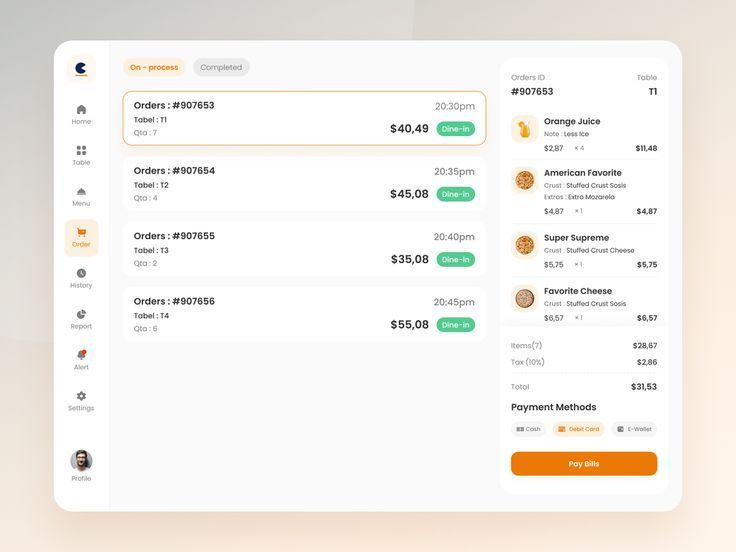
\includegraphics[width=0.9\linewidth]{HCI/images/restaurant_UI_1.jpg}
    \caption{}
    \label{fig:restUI1}
\end{figure}
\noindent
In the \cref{fig:restUI1} the design could fit restaurant systems user needs of

\subsubsection{name}
\begin{figure}[H]
    \centering
    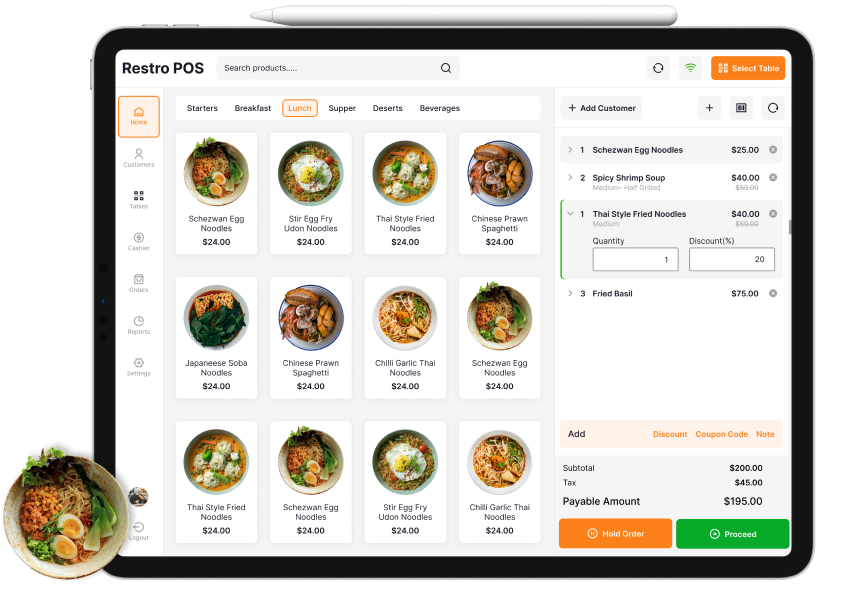
\includegraphics[width=0.9\linewidth]{HCI/images/restaurant_UI_2.png}
    \caption{}
    \label{fig:restUI2}
\end{figure}
\noindent
In the \cref{fig:restUI2} the design could fit restaurant PoS systems operators needs of 

\subsubsection{name}
\begin{figure}[H]
    \centering
    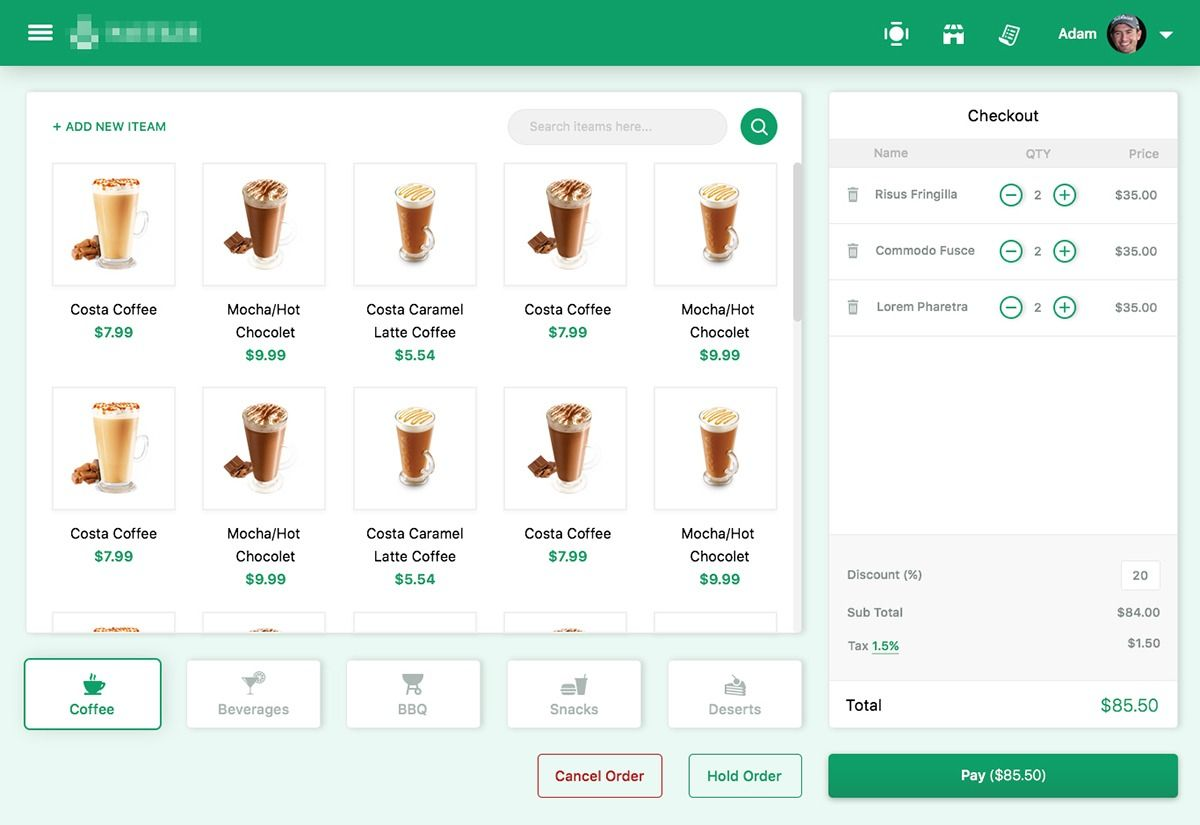
\includegraphics[width=0.9\linewidth]{HCI/images/restaurant_UI_3.jpg}
    \caption{}
    \label{fig:cafeUI}
\end{figure}
 \noindent
 In the \cref{fig:cafeUI} the design could fit PoS operators needs of cafe system like in the story \ref{Unknow language borders} of foreign employees Carlos and Juan. There's a search bar, but the UI is all english, so a slide bar for selecting a language could be added.

\subsubsection{name}


\subsubsection{name}


\end{document}
